\section{位置和轨迹的相对性}\label{sec:02.02}

在运动学中,最基本的概念是位置。由图\ref{fig:02.01}~看到。对于质点
$P$,相对于参考系$K$而言,它的位置矢量是$\vec{OP}$,即
\begin{equation*}
  \vec{OP}=x\vec{i}+y\vec{j}+z\vec{k}
\end{equation*}
同时,相对于参考系$K'$来说,它的位置矢量是$\vec{O'P}$,即
\begin{equation*}
  \vec{O'P}=x'\vec{i'}+y'\vec{j'}+z'\vec{k'}
\end{equation*}
\begin{figure}[h]
  \vspace{-1em}
  \centering
  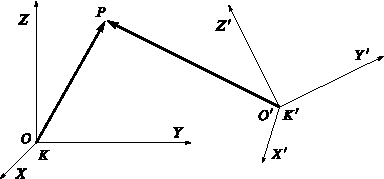
\includegraphics{figure/fig02.01}
  \caption{位置的相对性}
  \label{fig:02.01}
\end{figure}

\clearpage
可见同一质点的位置,对不同的参考系,可用不同的位置矢量来
描写,这就是位置描写中的相对性。

从描写质点位置来说,选用参考系$ K $或者$ K' $,是等价的。因
为参考系$K$及$K'$一旦选定,它们之间的关系就完全确定了。我们
知道了质点在参考系$K$中的位置坐标$\left(x,y,z\right)$,就可求得在参考
系$K'$中的位置坐标$\left(x',y',z'\right)$,反之亦然。用数学语言来说,
即$x,y,z$与$x',y',z'$之间有确定的变换关系:
\begin{align}
  \label{eqn:02.02.01}
   & \left\{\begin{array}{l}
              x'=x'\left(x, y, z\right) \\
              y'=y'\left(x, y, z\right) \\
              z'=z'\left(x, y, z\right)
            \end{array}\right.  \\
  \label{eqn:02.02.02}
   & \left\{\begin{array}{l}
              x=x\left(x', y', z'\right) \\
              y=y\left(x', y', z'\right) \\
              z=z\left(x', y', z'\right)
            \end{array}\right.
\end{align}
式\eqref{eqn:02.02.01}、\eqref{eqn:02.02.02}~称为坐标变换。

现在我们介绍几种物理学中常用的坐标变换。

\begin{wrapfigure}{r}{16em}
  \centering
  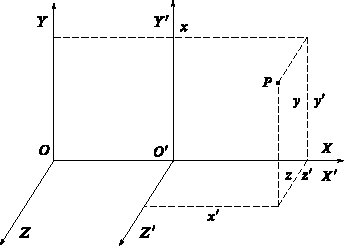
\includegraphics{figure/fig02.02}
  \caption{空间平移}
  \label{fig:02.02}
\end{wrapfigure}
\textsf{1. 坐标平移}

如图\ref{fig:02.02},参考系$K$及$K'$的$X$轴与$X'$轴重合,$Y$轴与$Y'$轴平行,
$Z$轴与$Z'$轴平行,原点$O$与$O'$相距$d$。若质点$P$的坐标在参考系$K$及$K'$中分别是$x,y,z$和
$x',y',z'$,显然,坐标变换是:
\begin{equation}\label{eqn:02.02.03}
  \left\{\begin{array}{l}
    x=x'+d \\
    y=y'   \\
    z=z'
  \end{array}\right.
\end{equation}

\begin{wrapfigure}{r}{15em}
  \centering
  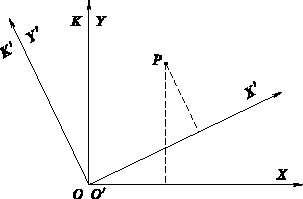
\includegraphics{figure/fig02.03}
  \caption{空间转动}
  \label{fig:02.03}
\end{wrapfigure}
\textsf{2. 坐标转动}

讨论平面问题时,取如图\ref{fig:02.03}~的参考系$K$及$K'$,它们的原点$O$与$O'$重合,参考
系$K'$的轴相对于参考系$ K $转动一个$\theta$角。质点$P$的位置坐标在参考系$K$,
$K'$中分别是$x,y,z$和$x',y',z'$。不难求出,此时的坐标变换是:
\begin{equation}\label{eqn:02.02.04}
  \left\{\begin{array}{l}
    x=x'\cos\theta-y'\sin\theta \\
    y=x'\sin\theta+y'\cos\theta
  \end{array}\right.
\end{equation}
或
\begin{equation*}
  \left\{\begin{array}{l}
    x'=x\cos\theta+y\sin\theta \\
    y'=-x\sin\theta+y\cos\theta
  \end{array}\right.
\end{equation*}

\begin{wrapfigure}{r}{15em}
  \centering
  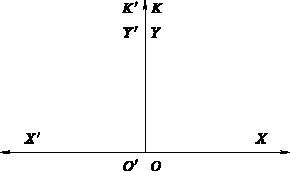
\includegraphics{figure/fig02.04}
  \caption{空间反演}
  \label{fig:02.04}
\end{wrapfigure}
\textsf{3. 空间反演}

如图\ref{fig:02.04},参考系$K$与$K'$的原点$O$与$O'$重合,$Y$轴与$Y'$轴重合,而$X$轴与
$X'$轴反向。这时,坐标变换是:
{\setlength{\mathindent}{2em}
\begin{equation}\label{eqn:02.02.05}
  \left\{\begin{array}{l}
    x=-x' \\
    y=y
  \end{array}\right.
\end{equation}}%

弄清了位置的相对性,关于轨迹的相对性也就不难理解了。

质点运动的轨迹,一般来说是一条空间曲线。对于一个质点
的轨迹,相对于参考系$ K $,我们可用曲线方程
\begin{equation}\label{eqn:02.02.06}
  \left\{\begin{array}{l}
    f_1\left(x,y,z\right)=0 \\
    f_2\left(x,y,z\right)=0
  \end{array}\right.
\end{equation}
来描写;也可相对于参考系$K'$,用曲线方程
\clearpage
\begin{equation}\label{eqn:02.02.07}
  \left\{\begin{array}{l}
    f'_1\left(x',y',z'\right)=0 \\
    f'_2\left(x',y',z'\right)=0
  \end{array}\right.
\end{equation}
来描写。一般说来,函数形式$f_1,f_2$和$f'_1,f'_2$是不相同的,这
就是轨迹的相对性。将式\eqref{eqn:02.02.02}~代入式\eqref{eqn:02.02.06},就可由$f$求得
$f'$;将式\eqref{eqn:02.02.01}~代入式\eqref{eqn:02.02.07},就可由$f'$求得$f$。

作为示例,我们讨论两个平面运动。有两个质点,它们相对
于参考系$K$的运动轨迹分别由下列曲线方程描写:
\begin{align}
  x-ky    & =0 \label{eqn:02.02.08}   \\
  x^2+y^2 & =r^2 \label{eqn:02.02.09}
\end{align}
式\eqref{eqn:02.02.08}~表示一直线运动,式\eqref{eqn:02.02.09}~表示中心在原点,半径
为$r$的一个圆周运动。

现在取另一参考系$K'$,它仅相对于参考系$K$转了一个$\theta$角。
我们把式\eqref{eqn:02.02.04}代入式\eqref{eqn:02.02.08},整理后得
{\setlength{\mathindent}{4em}
\begin{equation}\label{eqn:02.02.10}
  x'\left(\cos\theta - k\sin\theta\right)-y'\left(\sin\theta + k\cos\theta\right)=0
\end{equation}}%
式\eqref{eqn:02.02.10}~就是在参考系$K'$中所看到的第一个质点的轨迹方程,
它也是一条直线,但斜率与式\eqref{eqn:02.02.08}不同。

将式\eqref{eqn:02.02.04}~代入式\eqref{eqn:02.02.09},得
\begin{equation}\label{eqn:02.02.11}
  x'^2+y'^2=r^2
\end{equation}
由式\eqref{eqn:02.02.11}~看到,第二个质点的轨迹相对于参考系$K'$,也是中
心在原点。半径为$r$的圆。

如果一种运动轨迹相对于两参考系形状相同,而且它与两坐
标系的关系也一样,我们称这种特殊轨迹对于这一特定的坐标变
换具有不变性。用数学语言来说,当参考系$K$变到$K'$时,若轨迹
方程由
\begin{equation*}
  f\left(x,y,z\right)=0
\end{equation*}
变换成
\begin{equation*}
  f\left(x',y',z'\right)=0
\end{equation*}
它就是具有不变性的轨迹。由此可见,第一个质点轨迹相对于坐
标转动变换并不具有不变性,而第二个质点轨迹对于坐标转动变
换是有不变性的。

下面讨论涉及时间的变换,坐标系$K$及$K'$所用的时间$t$及$t'$
也可以是不相同的。最常遇到的一种时间变换,是所谓时间平移,
即$t=t'+t_0$,也就是$K$及$K'$的时间坐标的原点相差一常数$t_0$。
譬如,在参考系$K$中用东京时间,在参考系$K'$中用北京时间,
那么,常数$t_0$就等于1小时。

如果在参考系K中,轨迹函数是\vspace{-0.2em}
\\\null\hspace{6em}$x=x\left(t\right)$
\\\null\hspace{6em}$y=y\left(t\right)$
\\\null\hspace{6em}$z=z\left(t\right)$\\
我们很容易推知,在参考系$K'$中,轨迹函数是\vspace{-0.2em}
\\\null\hspace{6em}$x=x\left(t'+t_0\right)$
\\\null\hspace{6em}$y=y\left(t'+t_0\right)$
\\\null\hspace{6em}$z=z\left(t'+t_0\right)$

另一种时间变换在日常生活中不常见,但在物理上非常有用。
那就是\vspace{-0.5em}
\\\null\hspace{6em}$t=-t'$\\
它表示当$K$中的时间走向将来时,$K'$相应的时间却走向过去。因
此,称这种时间变换为时间倒转。

我们不难由参考系$K$中的轨迹函数\vspace{-0.2em}
\\\null\hspace{6em}$x=x\left(t\right)$
\\\null\hspace{6em}$y=y\left(t\right)$
\\\null\hspace{6em}$z=z\left(t\right)$\\
得到相应在参考系$K'$中的轨迹函数为\vspace{-0.2em}
\\\null\hspace{6em}$x=x\left(-t'\right)$
\\\null\hspace{6em}$y=y\left(-t'\right)$
\\\null\hspace{6em}$z=z\left(-t'\right)$

为了弄清时间倒转的物理意义,我们举一个直线运动的例子
(图\ref{fig:02.05})。质点沿$X$轴运动。在参考系$K$中看,$t=1$时,质点在$x_1$;
$t=2$时,在$x_2$;显然,质点是从左向右运动的。但在参考系$K'$中看,
质点在$x_1$时,$t'=-1$;在$x_2$时,$t'=-2$;由于时间$t'=-2$比$t'=-1$
早,而时间总是从过去向将来发展,因此,相对于参考系$K'$,质
点是从右向左运动的。
\begin{figure}[h]
  \centering
  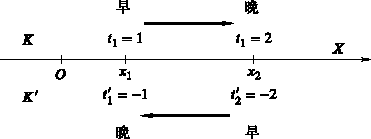
\includegraphics{figure/fig02.05}
  \caption{时间倒转}
  \label{fig:02.05}
\end{figure}
